\documentclass[t]{beamer}

\setlength {\marginparwidth }{2cm} 
\setlength {\parskip}{0cm} 
\usepackage{todonotes}
\usepackage{siunitx}
\usepackage{subcaption}
\usepackage{apacite} 	% Use APA Citation
\presetkeys{todonotes}{inline}{}
\beamertemplatenavigationsymbolsempty
\usefonttheme[onlymath]{serif}

\usepackage{algpseudocode}
\usepackage{enumitem,amssymb, yfonts, bm}
\newlist{todolist}{itemize}{2}
\setlist[todolist]{label=$\square$}
\usepackage{pifont}
\newcommand{\cmark}{\ding{51}}%
\newcommand{\xmark}{\ding{55}}%
\newcommand{\done}{\rlap{$\square$}{\raisebox{2pt}{\large\hspace{1pt}\cmark}}%
\hspace{-2.5pt}}

% \usetheme{AnnArbor}
% \usetheme{Antibes}
% \usetheme{Bergen}
% \usetheme{Berkeley}https://www.sharelatex.com/project/5b12e1a4f84b363f6f336dab
% \usetheme{Berlin}
% \usetheme{Boadilla}
% \usetheme{boxes}
\usetheme{CambridgeUS}
% \usetheme{Copenhagen}
%\usetheme{Darmstadt}
% \usetheme{default}
%\usetheme{Frankfurt}
%\usetheme{Goettingen}
% \usetheme{Hannover}
% \usetheme{Ilmenau}
% \usetheme{JuanLesPins}
\setlength{\parskip}{10pt}

% \newcommand*\vc[1]%
% {\begin{pmatrix}#1\end{pmatrix}}

\newcommand*\vc[1]%
{\left(\begin{array}{cccc}#1\end{array}\right)}


\newcommand\eqdef{\ \mathrel{\overset{\makebox[0pt]{\mbox{\normalfont\scriptsize\rmfamily def}}}{=}}\ }

\title[Eligibility propagation]{Improving eligibility propagation using Izhikevich neurons in a multilayer RSNN.\\\vspace{10pt}
\large{Presentation 5: Evaluation meeting 1}}

\author[Werner]{Werner~van~der~Veen\\\footnotesize\texttt({w.k.van.der.veen.2@student.rug.nl})}\date{\today}

\begin{document}

\begin{frame}
    \titlepage
\end{frame}

%======================================

%\begin{frame}
%    \tableofcontents
%\end{frame}

\small
\section{Project overview}
\begin{frame}{A quick project overview}
	Task: using eligibility propagation to classify phonemes.
	
	Challenges:
	\begin{itemize}[label=--]
		\item Desired bio-plasubility requires online and local learning rules.
		\item Spiking and reccurent network: no good learning algorithm yet.
	\end{itemize}
	
	My own contribution: investigate the benefits of
	\begin{itemize}[label=--]
		\item stacking multiple recurrent layers
		\item using Izhikevich neurons
		\item various regularization methods
	\end{itemize}
		
\end{frame}

\section{Background}
\begin{frame}{Original network architecture}
	\begin{figure}[!ht]
		


\tikzset{every picture/.style={line width=0.75pt}} %set default line width to 0.75pt        

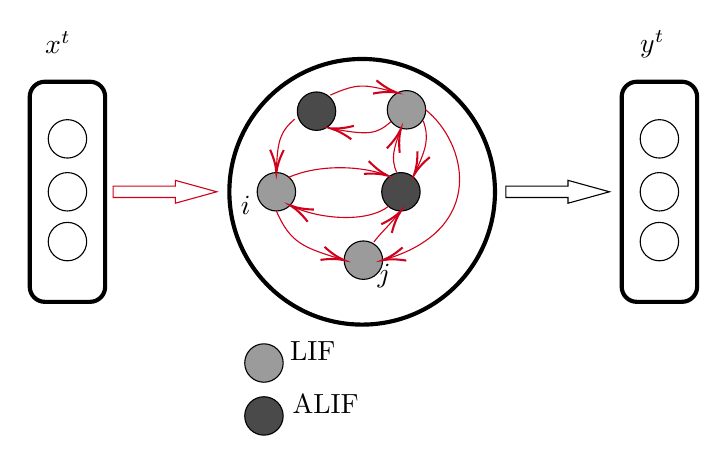
\begin{tikzpicture}[x=0.75pt,y=0.75pt,yscale=-1,xscale=1]
%uncomment if require: \path (0,300); %set diagram left start at 0, and has height of 300

%Rounded Rect [id:dp5125213371166828] 
\draw  [line width=1.5]  (20,112.05) .. controls (20,108.03) and (23.25,104.78) .. (27.27,104.78) -- (49.07,104.78) .. controls (53.08,104.78) and (56.33,108.03) .. (56.33,112.05) -- (56.33,203.55) .. controls (56.33,207.57) and (53.08,210.82) .. (49.07,210.82) -- (27.27,210.82) .. controls (23.25,210.82) and (20,207.57) .. (20,203.55) -- cycle ;
%Shape: Circle [id:dp1036864356471725] 
\draw   (28.91,181.8) .. controls (28.91,176.69) and (33.06,172.55) .. (38.17,172.55) .. controls (43.28,172.55) and (47.42,176.69) .. (47.42,181.8) .. controls (47.42,186.91) and (43.28,191.05) .. (38.17,191.05) .. controls (33.06,191.05) and (28.91,186.91) .. (28.91,181.8) -- cycle ;
%Shape: Circle [id:dp6658728805120719] 
\draw   (28.91,132.3) .. controls (28.91,127.19) and (33.06,123.05) .. (38.17,123.05) .. controls (43.28,123.05) and (47.42,127.19) .. (47.42,132.3) .. controls (47.42,137.41) and (43.28,141.55) .. (38.17,141.55) .. controls (33.06,141.55) and (28.91,137.41) .. (28.91,132.3) -- cycle ;
%Right Arrow [id:dp741109303104662] 
\draw  [color={rgb, 255:red, 208; green, 2; blue, 27 }  ,draw opacity=1 ] (60.17,155.05) -- (90.13,155.05) -- (90.13,152.29) -- (110.11,157.8) -- (90.13,163.31) -- (90.13,160.55) -- (60.17,160.55) -- cycle ;
%Shape: Circle [id:dp6585629105990938] 
\draw  [color={rgb, 255:red, 0; green, 0; blue, 0 }  ,draw opacity=1 ][line width=1.5]  (116.17,157.8) .. controls (116.17,122.46) and (144.82,93.81) .. (180.15,93.81) .. controls (215.49,93.81) and (244.14,122.46) .. (244.14,157.8) .. controls (244.14,193.14) and (215.49,221.79) .. (180.15,221.79) .. controls (144.82,221.79) and (116.17,193.14) .. (116.17,157.8) -- cycle ;
%Shape: Circle [id:dp741227979850853] 
\draw  [fill={rgb, 255:red, 74; green, 74; blue, 74 }  ,fill opacity=1 ] (148.91,118.97) .. controls (148.91,113.86) and (153.06,109.71) .. (158.17,109.71) .. controls (163.28,109.71) and (167.42,113.86) .. (167.42,118.97) .. controls (167.42,124.08) and (163.28,128.22) .. (158.17,128.22) .. controls (153.06,128.22) and (148.91,124.08) .. (148.91,118.97) -- cycle ;
%Shape: Circle [id:dp7307755920673902] 
\draw  [fill={rgb, 255:red, 155; green, 155; blue, 155 }  ,fill opacity=1 ] (192.25,118.3) .. controls (192.25,113.19) and (196.39,109.05) .. (201.5,109.05) .. controls (206.61,109.05) and (210.75,113.19) .. (210.75,118.3) .. controls (210.75,123.41) and (206.61,127.55) .. (201.5,127.55) .. controls (196.39,127.55) and (192.25,123.41) .. (192.25,118.3) -- cycle ;
%Shape: Circle [id:dp39480228938683437] 
\draw  [fill={rgb, 255:red, 155; green, 155; blue, 155 }  ,fill opacity=1 ] (129.58,157.8) .. controls (129.58,152.69) and (133.72,148.55) .. (138.83,148.55) .. controls (143.94,148.55) and (148.09,152.69) .. (148.09,157.8) .. controls (148.09,162.91) and (143.94,167.05) .. (138.83,167.05) .. controls (133.72,167.05) and (129.58,162.91) .. (129.58,157.8) -- cycle ;
%Shape: Circle [id:dp707851840639744] 
\draw  [fill={rgb, 255:red, 74; green, 74; blue, 74 }  ,fill opacity=1 ] (189.58,157.8) .. controls (189.58,152.69) and (193.72,148.55) .. (198.83,148.55) .. controls (203.94,148.55) and (208.09,152.69) .. (208.09,157.8) .. controls (208.09,162.91) and (203.94,167.05) .. (198.83,167.05) .. controls (193.72,167.05) and (189.58,162.91) .. (189.58,157.8) -- cycle ;
%Shape: Circle [id:dp5633766668791496] 
\draw  [fill={rgb, 255:red, 155; green, 155; blue, 155 }  ,fill opacity=1 ] (171.49,190.75) .. controls (171.49,185.64) and (175.64,181.49) .. (180.75,181.49) .. controls (185.86,181.49) and (190,185.64) .. (190,190.75) .. controls (190,195.86) and (185.86,200) .. (180.75,200) .. controls (175.64,200) and (171.49,195.86) .. (171.49,190.75) -- cycle ;
%Curve Lines [id:da5654601008343274] 
\draw [color={rgb, 255:red, 208; green, 2; blue, 27 }  ,draw opacity=1 ]   (138.83,167.05) .. controls (145.61,182.74) and (152.21,184.72) .. (169.83,190.23) ;
\draw [shift={(171.49,190.75)}, rotate = 197.41] [color={rgb, 255:red, 208; green, 2; blue, 27 }  ,draw opacity=1 ][line width=0.75]    (10.93,-3.29) .. controls (6.95,-1.4) and (3.31,-0.3) .. (0,0) .. controls (3.31,0.3) and (6.95,1.4) .. (10.93,3.29)   ;
%Curve Lines [id:da8424508537757602] 
\draw [color={rgb, 255:red, 208; green, 2; blue, 27 }  ,draw opacity=1 ]   (144.81,150.81) .. controls (157.8,145.08) and (176.99,144.82) .. (190.54,149.34) ;
\draw [shift={(192.41,150.01)}, rotate = 200.92000000000002] [color={rgb, 255:red, 208; green, 2; blue, 27 }  ,draw opacity=1 ][line width=0.75]    (10.93,-3.29) .. controls (6.95,-1.4) and (3.31,-0.3) .. (0,0) .. controls (3.31,0.3) and (6.95,1.4) .. (10.93,3.29)   ;
%Curve Lines [id:da8098070733054574] 
\draw [color={rgb, 255:red, 208; green, 2; blue, 27 }  ,draw opacity=1 ]   (192.81,164.81) .. controls (183.21,172.49) and (161.08,171.32) .. (147.29,165.2) ;
\draw [shift={(145.61,164.41)}, rotate = 386.57] [color={rgb, 255:red, 208; green, 2; blue, 27 }  ,draw opacity=1 ][line width=0.75]    (10.93,-3.29) .. controls (6.95,-1.4) and (3.31,-0.3) .. (0,0) .. controls (3.31,0.3) and (6.95,1.4) .. (10.93,3.29)   ;
%Curve Lines [id:da5891979583346552] 
\draw [color={rgb, 255:red, 208; green, 2; blue, 27 }  ,draw opacity=1 ]   (164.81,111.21) .. controls (177.87,105.45) and (180.97,105.96) .. (195,109.55) ;
\draw [shift={(196.81,110.01)}, rotate = 194.38] [color={rgb, 255:red, 208; green, 2; blue, 27 }  ,draw opacity=1 ][line width=0.75]    (10.93,-3.29) .. controls (6.95,-1.4) and (3.31,-0.3) .. (0,0) .. controls (3.31,0.3) and (6.95,1.4) .. (10.93,3.29)   ;
%Curve Lines [id:da264987914027079] 
\draw [color={rgb, 255:red, 208; green, 2; blue, 27 }  ,draw opacity=1 ]   (196.76,148.41) .. controls (193.82,141.79) and (195.61,136.52) .. (198.1,129.49) ;
\draw [shift={(198.76,127.61)}, rotate = 469.29] [color={rgb, 255:red, 208; green, 2; blue, 27 }  ,draw opacity=1 ][line width=0.75]    (10.93,-3.29) .. controls (6.95,-1.4) and (3.31,-0.3) .. (0,0) .. controls (3.31,0.3) and (6.95,1.4) .. (10.93,3.29)   ;
%Curve Lines [id:da17823983207616156] 
\draw [color={rgb, 255:red, 208; green, 2; blue, 27 }  ,draw opacity=1 ]   (147.61,122.81) .. controls (141.08,128.57) and (139.35,132.49) .. (138.89,146.71) ;
\draw [shift={(138.83,148.55)}, rotate = 271.38] [color={rgb, 255:red, 208; green, 2; blue, 27 }  ,draw opacity=1 ][line width=0.75]    (10.93,-3.29) .. controls (6.95,-1.4) and (3.31,-0.3) .. (0,0) .. controls (3.31,0.3) and (6.95,1.4) .. (10.93,3.29)   ;
%Curve Lines [id:da7421559076195556] 
\draw [color={rgb, 255:red, 208; green, 2; blue, 27 }  ,draw opacity=1 ]   (185.81,182.03) .. controls (188.45,178.27) and (191.43,175.92) .. (197.61,168.53) ;
\draw [shift={(198.83,167.05)}, rotate = 489.31] [color={rgb, 255:red, 208; green, 2; blue, 27 }  ,draw opacity=1 ][line width=0.75]    (10.93,-3.29) .. controls (6.95,-1.4) and (3.31,-0.3) .. (0,0) .. controls (3.31,0.3) and (6.95,1.4) .. (10.93,3.29)   ;
%Curve Lines [id:da4256075721549528] 
\draw [color={rgb, 255:red, 208; green, 2; blue, 27 }  ,draw opacity=1 ]   (194.01,124.01) .. controls (187.45,129.8) and (183.87,130.75) .. (166.73,127.57) ;
\draw [shift={(164.81,127.21)}, rotate = 370.84000000000003] [color={rgb, 255:red, 208; green, 2; blue, 27 }  ,draw opacity=1 ][line width=0.75]    (10.93,-3.29) .. controls (6.95,-1.4) and (3.31,-0.3) .. (0,0) .. controls (3.31,0.3) and (6.95,1.4) .. (10.93,3.29)   ;
%Shape: Circle [id:dp8922241675489593] 
\draw  [fill={rgb, 255:red, 74; green, 74; blue, 74 }  ,fill opacity=1 ] (123.58,265.8) .. controls (123.58,260.69) and (127.72,256.55) .. (132.83,256.55) .. controls (137.94,256.55) and (142.09,260.69) .. (142.09,265.8) .. controls (142.09,270.91) and (137.94,275.05) .. (132.83,275.05) .. controls (127.72,275.05) and (123.58,270.91) .. (123.58,265.8) -- cycle ;
%Shape: Circle [id:dp07237313980777427] 
\draw  [fill={rgb, 255:red, 155; green, 155; blue, 155 }  ,fill opacity=1 ] (123.58,240.3) .. controls (123.58,235.19) and (127.72,231.05) .. (132.83,231.05) .. controls (137.94,231.05) and (142.09,235.19) .. (142.09,240.3) .. controls (142.09,245.41) and (137.94,249.55) .. (132.83,249.55) .. controls (127.72,249.55) and (123.58,245.41) .. (123.58,240.3) -- cycle ;
%Right Arrow [id:dp7348532029334156] 
\draw  [color={rgb, 255:red, 0; green, 0; blue, 0 }  ,draw opacity=1 ] (249.37,155.05) -- (279.33,155.05) -- (279.33,152.29) -- (299.31,157.8) -- (279.33,163.31) -- (279.33,160.55) -- (249.37,160.55) -- cycle ;
%Shape: Circle [id:dp026235667443113897] 
\draw   (28.91,157.8) .. controls (28.91,152.69) and (33.06,148.55) .. (38.17,148.55) .. controls (43.28,148.55) and (47.42,152.69) .. (47.42,157.8) .. controls (47.42,162.91) and (43.28,167.05) .. (38.17,167.05) .. controls (33.06,167.05) and (28.91,162.91) .. (28.91,157.8) -- cycle ;
%Rounded Rect [id:dp8136688725026966] 
\draw  [line width=1.5]  (305.2,112.05) .. controls (305.2,108.03) and (308.45,104.78) .. (312.47,104.78) -- (334.27,104.78) .. controls (338.28,104.78) and (341.53,108.03) .. (341.53,112.05) -- (341.53,203.55) .. controls (341.53,207.57) and (338.28,210.82) .. (334.27,210.82) -- (312.47,210.82) .. controls (308.45,210.82) and (305.2,207.57) .. (305.2,203.55) -- cycle ;
%Shape: Circle [id:dp11133772958248556] 
\draw   (314.11,181.8) .. controls (314.11,176.69) and (318.26,172.55) .. (323.37,172.55) .. controls (328.48,172.55) and (332.62,176.69) .. (332.62,181.8) .. controls (332.62,186.91) and (328.48,191.05) .. (323.37,191.05) .. controls (318.26,191.05) and (314.11,186.91) .. (314.11,181.8) -- cycle ;
%Shape: Circle [id:dp9075431994144578] 
\draw   (314.11,132.3) .. controls (314.11,127.19) and (318.26,123.05) .. (323.37,123.05) .. controls (328.48,123.05) and (332.62,127.19) .. (332.62,132.3) .. controls (332.62,137.41) and (328.48,141.55) .. (323.37,141.55) .. controls (318.26,141.55) and (314.11,137.41) .. (314.11,132.3) -- cycle ;
%Shape: Circle [id:dp30918690373576596] 
\draw   (314.11,157.8) .. controls (314.11,152.69) and (318.26,148.55) .. (323.37,148.55) .. controls (328.48,148.55) and (332.62,152.69) .. (332.62,157.8) .. controls (332.62,162.91) and (328.48,167.05) .. (323.37,167.05) .. controls (318.26,167.05) and (314.11,162.91) .. (314.11,157.8) -- cycle ;
%Curve Lines [id:da005449794705521871] 
\draw [color={rgb, 255:red, 208; green, 2; blue, 27 }  ,draw opacity=1 ]   (210.75,118.3) .. controls (230.55,134.14) and (240.61,175.62) .. (191.51,190.31) ;
\draw [shift={(190,190.75)}, rotate = 344.28999999999996] [color={rgb, 255:red, 208; green, 2; blue, 27 }  ,draw opacity=1 ][line width=0.75]    (10.93,-3.29) .. controls (6.95,-1.4) and (3.31,-0.3) .. (0,0) .. controls (3.31,0.3) and (6.95,1.4) .. (10.93,3.29)   ;
%Curve Lines [id:da9608524955121955] 
\draw [color={rgb, 255:red, 208; green, 2; blue, 27 }  ,draw opacity=1 ]   (209.56,123.61) .. controls (212.6,131.97) and (210.95,137.08) .. (205.97,147.86) ;
\draw [shift={(205.16,149.61)}, rotate = 295.02] [color={rgb, 255:red, 208; green, 2; blue, 27 }  ,draw opacity=1 ][line width=0.75]    (10.93,-3.29) .. controls (6.95,-1.4) and (3.31,-0.3) .. (0,0) .. controls (3.31,0.3) and (6.95,1.4) .. (10.93,3.29)   ;

% Text Node
\draw (120.4,158.8) node [anchor=north west][inner sep=0.75pt]    {$i$};
% Text Node
\draw (186.35,191.5) node [anchor=north west][inner sep=0.75pt]    {$j$};
% Text Node
\draw (145.37,254.3) node [anchor=north west][inner sep=0.75pt]   [align=left] {ALIF};
% Text Node
\draw (144.17,228.8) node [anchor=north west][inner sep=0.75pt]   [align=left] {LIF};
% Text Node
\draw (26.17,79.4) node [anchor=north west][inner sep=0.75pt]    {$x^{t}$};
% Text Node
\draw (312.87,79) node [anchor=north west][inner sep=0.75pt]    {$y^{t}$};


\end{tikzpicture}

	\end{figure}
\end{frame}



\begin{frame}{The e-prop learning algorithm -- Main equation}
	
	\begin{align*}
		\frac{dE}{dW_{ji}} 
		&= \sum_tL_j^t \cdot e_{ji}^t
	\end{align*}
	
	\begin{figure}[!ht]
		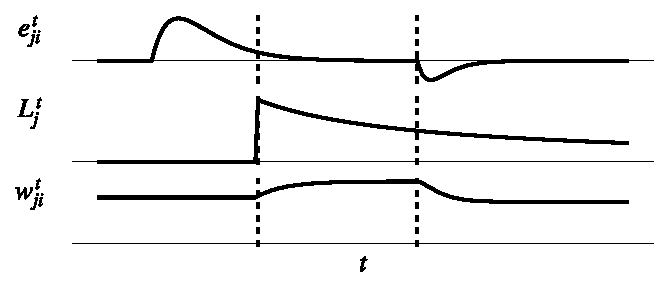
\includegraphics[width=0.8\linewidth]{eligibility.pdf}
	\end{figure}
	
\end{frame}

\begin{frame}{The e-prop learning algorithm -- proof}
	
	\begin{align*}
		\frac{dE}{dW_{ji}} 
		&= \sum_tL_j^t \cdot e_{ji}^t
	\end{align*}
	
	\begin{equation*}
L^t_j \eqdef \frac{dE}{dz^t_j}
\end{equation*}

	\begin{equation*}
e^t_{ji} \eqdef \frac{\partial z_j^t}{\partial\mathbf{h}_j^t}\underbrace{\sum_{t'\leq t}\frac{\partial\mathbf{h}^t_j}{\partial\mathbf{h}_j^{t-1}} \cdots \frac{\partial\mathbf{h}_j^{t'+1}}{\partial\mathbf{h}_j^{t'}}\cdot\frac{\partial\mathbf{h}_j^{t'}}{\partial W_{ji}}}_{\eqdef \bm{\varepsilon}_{ji}^t}
\end{equation*}
	
	
\end{frame}

\begin{frame}{The e-prop learning algorithm -- Original LIF}
	
	\begin{figure}[!ht]
		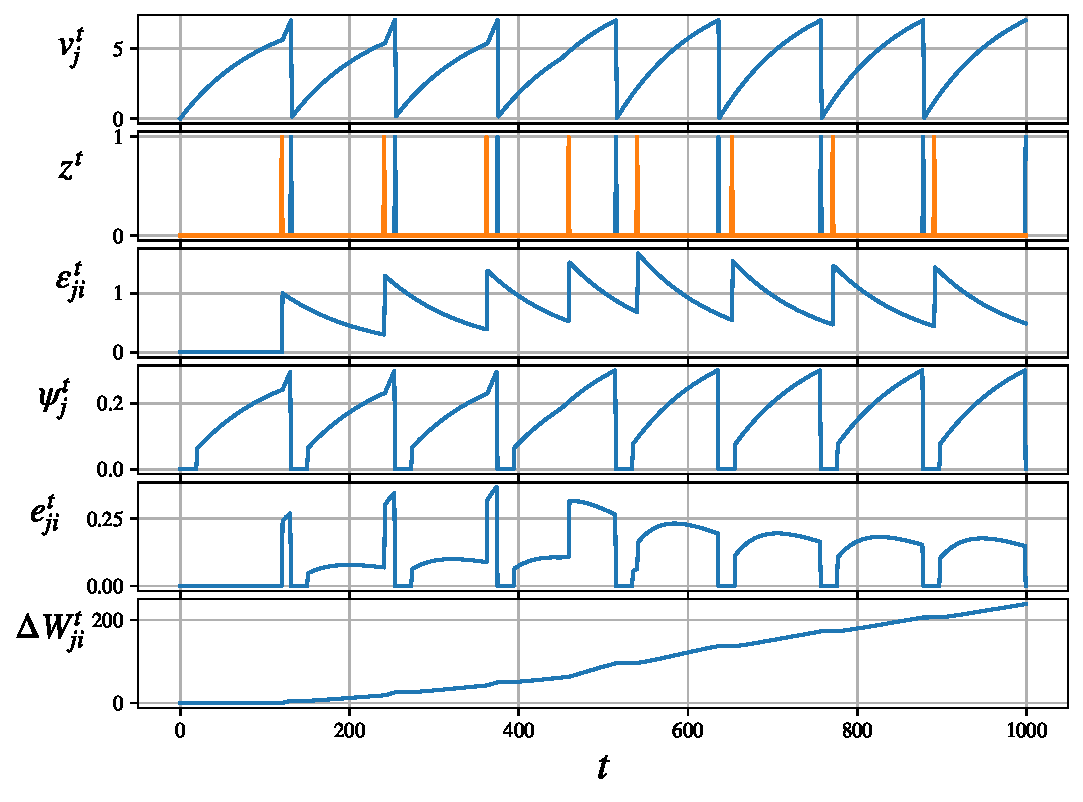
\includegraphics[width=0.8\linewidth]{eprop_demo_bellec.pdf}
	\end{figure}
	
\end{frame}

\begin{frame}{Previous results}
\tiny{
Bellec, G., Scherr, F., Subramoney, A., Hajek, E., Salaj, D., Legenstein, R., \& Maass, W. (2020). A solution to the learning dilemma for recurrent networks of spiking neurons.}
	
\begin{figure}[!ht]
		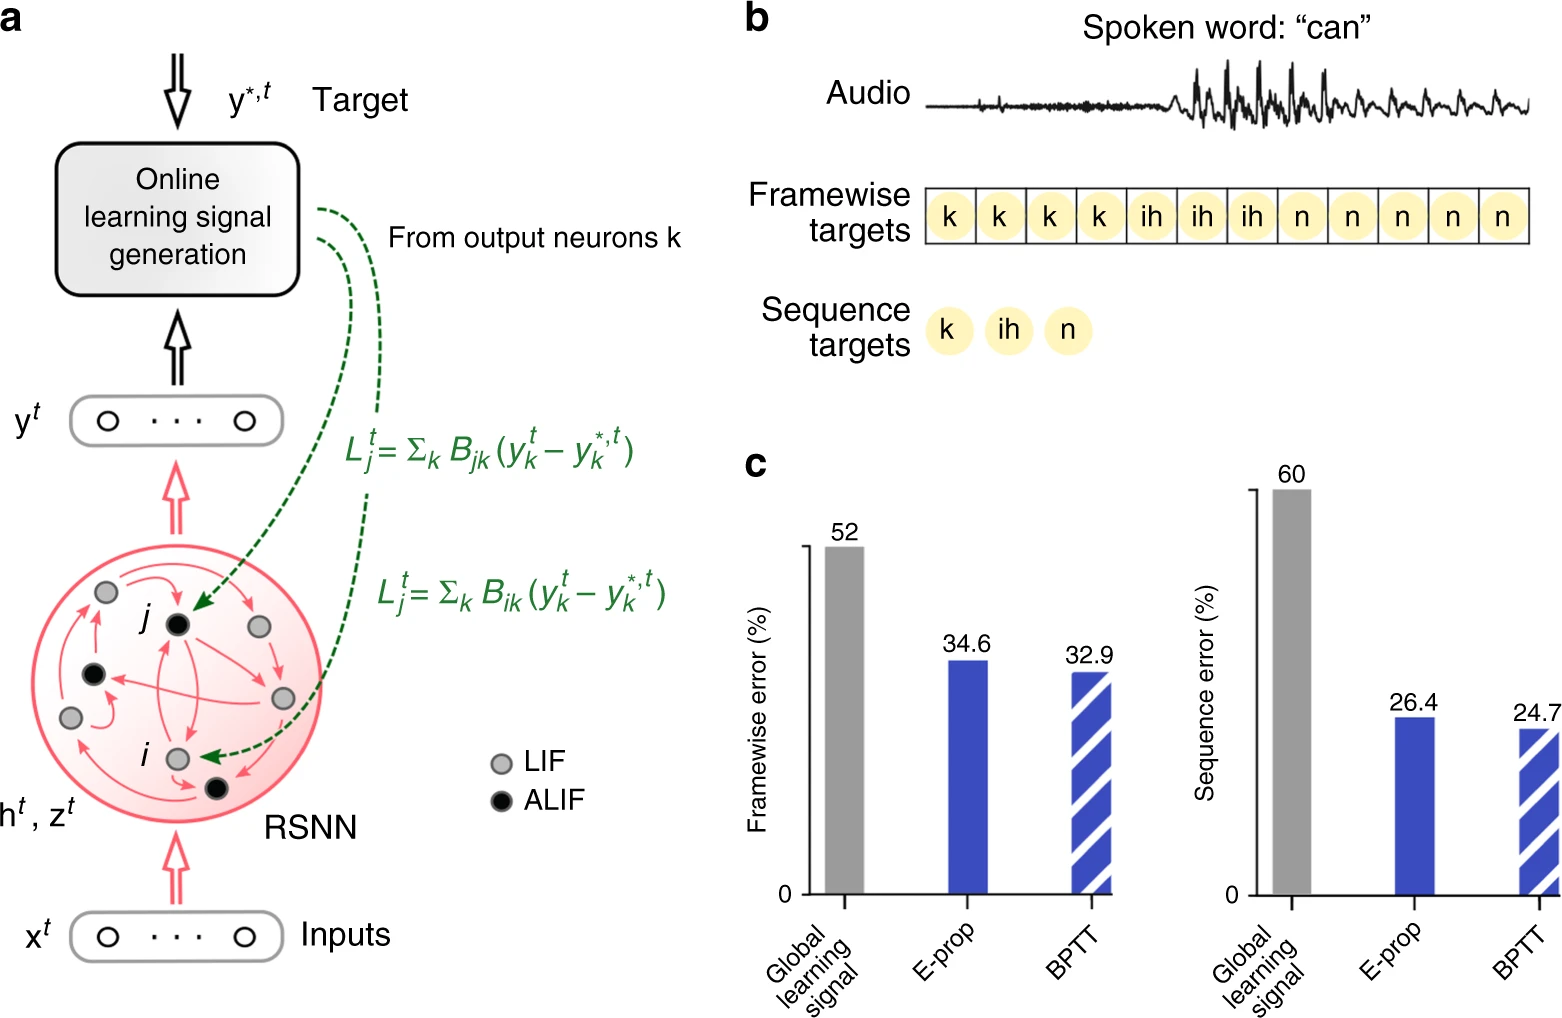
\includegraphics[width=0.8\linewidth]{timitperformance.png}
	\end{figure}
	
\end{frame}

\begin{frame}{The e-prop learning algorithm -- STDP-corrected LIF}
\tiny{
Traub, M., Butz, M. V., Baayen, R. H., \& Otte, S. (2020, September). Learning Precise Spike Timings with Eligibility Traces. In International Conference on Artificial Neural Networks (pp. 659-669). Springer, Cham.}

	\begin{figure}[!ht]
		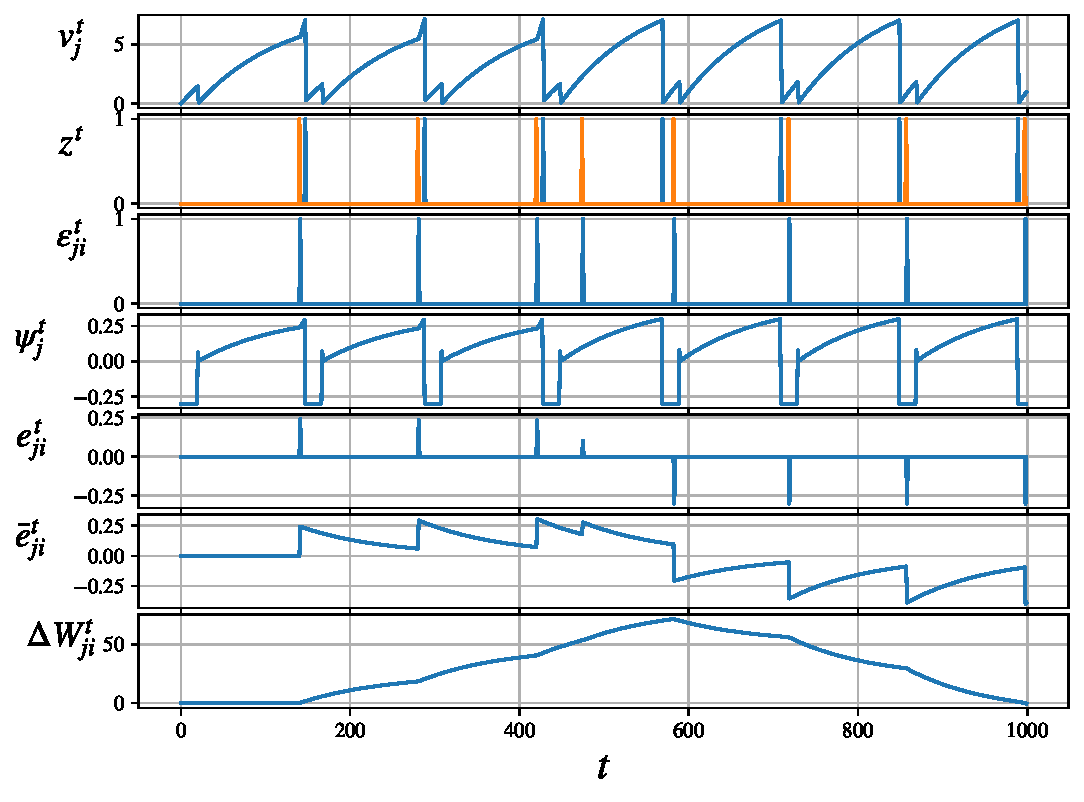
\includegraphics[width=0.78\linewidth]{demo_traubfix.pdf}
	\end{figure}
	
\end{frame}

\section{Proposal}
\begin{frame}{My proposed contribution}
\begin{itemize}[label=--]
\item Implement the algorithm in a \emph{multi-layer} SRNN.
	\begin{figure}[!ht]
		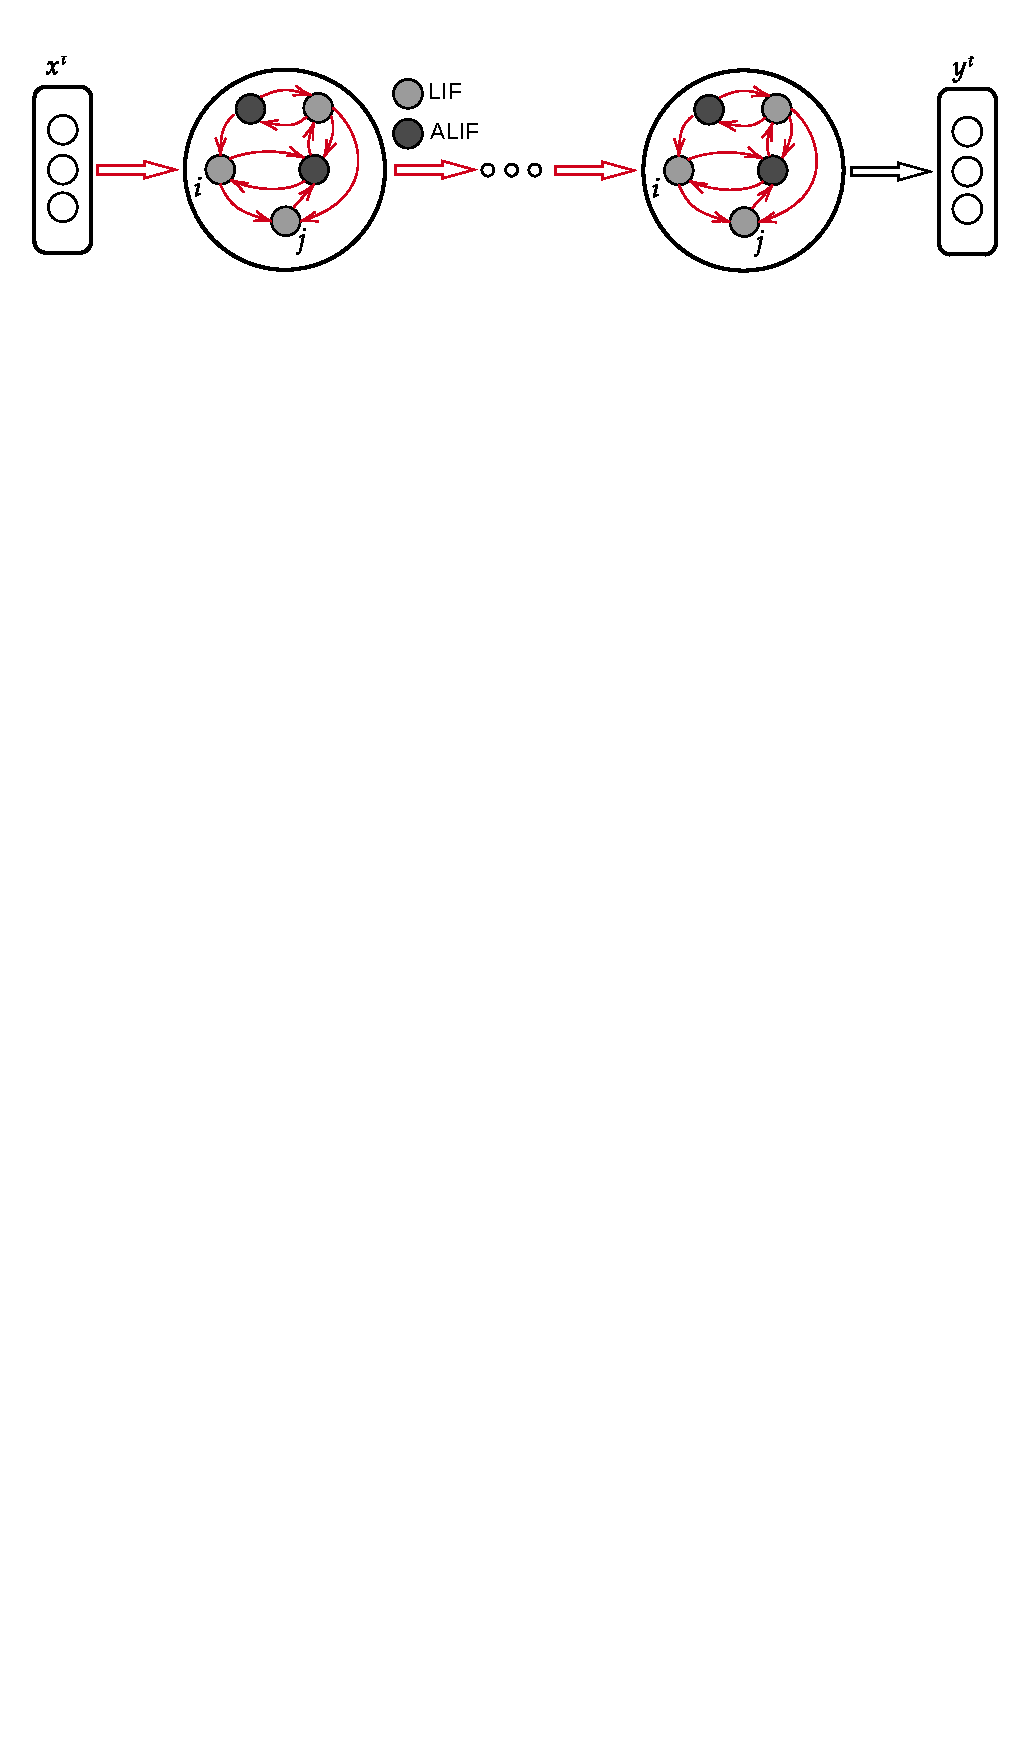
\includegraphics[clip, trim=0cm 25cm 0cm 0cm, width=0.667\linewidth]{BellecDiagramML.pdf}  %lbrt
	\end{figure}
\item Examine model desgns such as neuron type (e.g. Izhikevich); synaptic delay; and regularization such as metaplasticity and synaptic scaling.
\end{itemize}
	
\end{frame}

\section{Current state}
\begin{frame}{Work done so far}
	\begin{todolist}

    \item[\done] Implement Bellec's model with
    \begin{todolist}
    	\item[\done] 1-layer e-prop RSNN with ALIF neurons;
    	\item[\done] TIMIT conversion to 13 MFCCs and their first and second derivatives;
    	\item[\done] $L^2$ and firing rate regularization;
    	\item[\done] Adam optimizer;
    \item[\done] Bidirectional network.
    \end{todolist}
    \item Obtain Bellec's performance;
    \item Analyze effects of
    \begin{todolist}
    	\item N-layered network;
    \item Izhikevich neurons;
    	\item Metaplasticity;
    	\item Synaptic scaling;
    	\item Synaptic delays.
    \end{todolist}
  \end{todolist}
  
\begin{tikzpicture}[remember picture,overlay]
    \node[xshift=-2cm,yshift=-6.5cm] at (current page.north east) {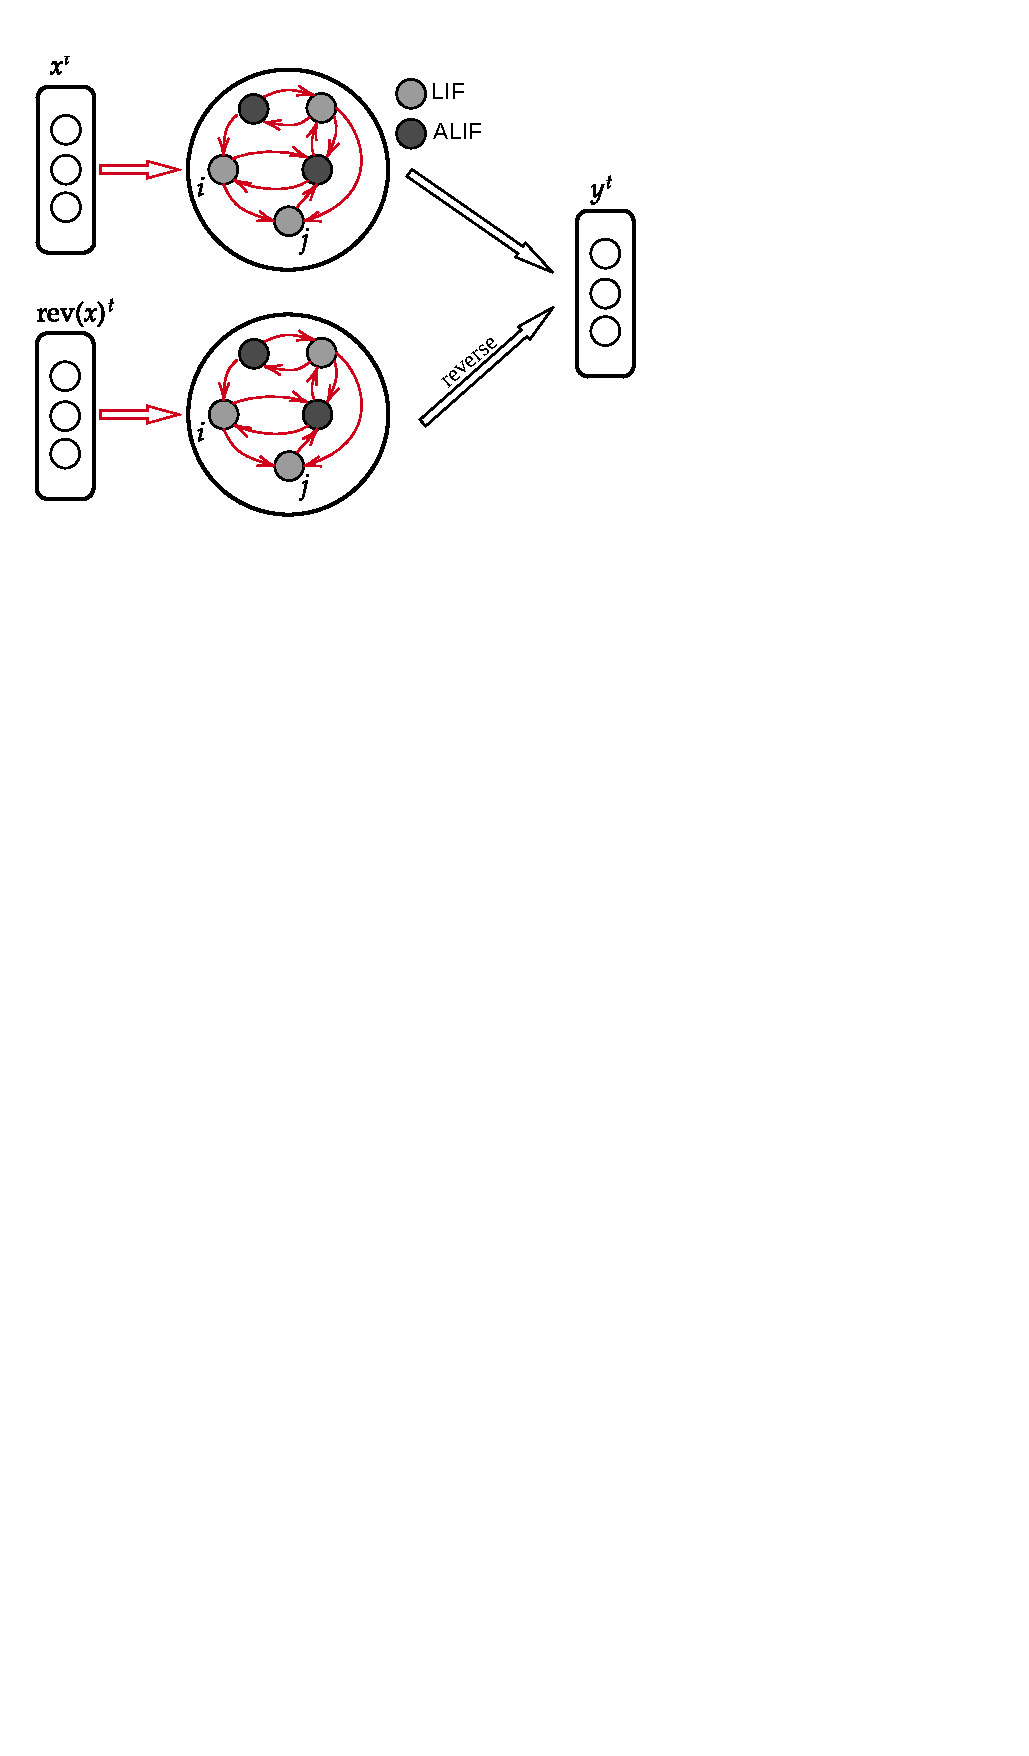
\includegraphics[clip, trim=0cm 21cm 0cm 0cm, width=0.8\linewidth]{BellecDiagramBi.pdf}};
\end{tikzpicture}
\end{frame}


\begin{frame}{Current observations}

\begin{itemize}[label=--]
\item \[\lim_{e \to \infty} W^e_\textrm{out}  = \mathbf{0}\]
\[\lim_{e \to \infty} b^e_\textrm{out}  = \mathbf{0}\]
\item Spike frequency normal but heavily affected by weight initialization. Weights in order of $[0, \frac{2}{N}]$ work well, where $N$ is layer size.
\end{itemize}
\end{frame}




\end{document}
